% Chapter 5 -- Five use cases: data, rusty-SUNDIALS and LeanFlow
% All numerical values in this chapter come from the JSON outputs of the scripts code/ch5_U*.py
% (run on 2026-10-26) or from the primary files cited; none is typed in by hand.
\chapter{Five use cases: data, rusty-SUNDIALS and LeanFlow}\label{ch5:chapitre}\label{ch5:debut}

The previous chapters built statements: theorems checked by the Lean kernel, their human proofs and their
hypotheses. This chapter puts them to work on five real systems:
\begin{itemize}
\item dipolar excitons in a transition-metal dichalcogenide heterobilayer;
\item planar Yukawa crystals, as in dusty plasmas and colloids;
\item the structure of superfluid helium;
\item a shell model of turbulence;
\item the fixation of a mutation in a population.
\end{itemize}
Every case follows the same plan, and you can redo all of it: each section ends with a script in
\texttt{code/} that downloads or checks the data, runs the solver and produces the figure printed here.

\begin{warnbox}[: what this chapter is, and what it is not]
\begin{itemize}
\item The five cases \emph{illustrate} theorems; they do not \emph{prove} them. A simulation is
Tier~X: it never supports a claim.
\item The datasets provide orders of magnitude, realistic initial conditions or spectra. None
of them tests a Tier~A theorem, and each time we say what it does not show.
\item All results reused here were produced by AI agents (Claude) under the author's direction,
then audited by a separate AI agent. The computations redone for this chapter are checked only by the agent that
produced them: the reruns, the Python controls, the sequence statistics and the LeanFlow certificates. No
human has audited these results.
\item The statements about the triangular lattice (cases U1 and U2) are \emph{conditional} on the upstream theorem
\lean{universal_energy_minimum} of openai/math, which is AI-generated and has not been peer reviewed.
\end{itemize}
\end{warnbox}

\section{Common method}\label{ch5:methode}

\paragraph{The four ingredients.} Each case combines four ingredients:
\begin{enumerate}
\item \textbf{A question} from physics or biology, asked before looking at the numbers.
\item \textbf{A theorem}, with its tier (A, L, C or X), its Lean name and its DOI. The tier refers to
the Lean statement, never to its physical reading.
\item \textbf{Data}. For each dataset we give the identifier, the exact revision (a 40-character \texttt{git}
hash), the licence as displayed on the dataset card, and the \texttt{sha256} digest of the
file used. When no Hugging Face dataset exists, we say so.
\item \textbf{A numerical method}. It relies on rusty-SUNDIALS, a Rust rewrite of SUNDIALS: CVODE
(BDF formulas) for stiff differential equations, plus physics modules (\texttt{qf-*}). When
a value must be certified exactly, we go through LeanFlow, which turns a rational numerical claim
into a Lean file, has it checked by the kernel and audits its axioms.
\end{enumerate}

\paragraph{The control rule.} Before a number is published, every experiment runs at least one
\emph{positive control} and one \emph{negative control}:
\begin{itemize}
\item the positive control is a case whose answer is known, and the code must recover it;
\item the negative control is a case that is wrong or deliberately broken, and the code must reject it.
\end{itemize}
A test that has never failed on a negative control has tested nothing. The five scripts terminate with exit
code~1 if a control does not behave as expected.

\paragraph{Reproducing.} The binaries come from a working copy of rusty-SUNDIALS. It contains the merged crates
\texttt{qf-yukawa-crystal}, \texttt{qf-shell-cascade}, \texttt{qf-gpe2d} and \texttt{qf-popgen}:
\begin{itemize}
\item branch \texttt{textbook2/ch5-cas-usage-2026-10-26};
\item based on commit \texttt{cda9a9057ec16820f2e16b560cc0e63cf7eb05b9}.
\end{itemize}
They are built and used as follows:
\begin{lstlisting}[language={}]
CARGO_TARGET_DIR=~/rusty-target-ar cargo build --release -j 2 --offline \
   -p qf-yukawa-crystal -p qf-shell-cascade -p qf-popgen
python -I code/ch5_U1_dipolar.py  sortie_U1 --bin ~/rusty-target-ar/release
python -I code/ch5_U5_fixation.py sortie_U5 --bin ~/rusty-target-ar/release
\end{lstlisting}
The option \texttt{-I} isolates the interpreter: it ignores \texttt{PYTHONPATH} and the current directory, which
protects against a planted file in a folder of downloaded data. Each script prints a summary and writes a file
\texttt{ch5\_U*\_result.json}. The numbers in this chapter are those of these files.

We first reran the binaries inside the working copy itself: there, the outputs overwrite the
published records. \texttt{git diff} then shows that the recomputed files are bit-for-bit identical
to the records, only the run times differing:
\begin{itemize}
\item \texttt{lattice\_gaps.jsonl} and \texttt{references.jsonl} (U1);
\item \texttt{exact\_refs.jsonl} and \texttt{exact\_relax\_kappa2\_a0\_f0.jsonl} (U2);
\item \texttt{linear\_response.json} of \texttt{qf-gpe2d} (U3);
\item \texttt{sigma3\_study.json} (U4);
\item \texttt{results.jsonl} (U5).
\end{itemize}

\begin{table}[ht]\centering\small
\caption{The five use cases at a glance.}\label{ch5:tab:resume}
\begin{tabular}{p{2.2cm}p{3.6cm}p{3.4cm}p{4.2cm}}\toprule
case & theorem (tier) & data & numerics\\\midrule
U1 excitons & optimality of the triangular lattice for $2(1/r-1/\sqrt{r^2+d^2})$ (A, conditional) &
JARVIS-DFT (HF) & exact Ewald, CVODE \\
U2 Yukawa & same for $e^{-\kappa r}/r$ (A, conditional) & OC20 (HF), disorder only & exact energies, CVODE\\
U3 helium & $S_B(k)\le\sqrt{k/2k^*}$ (A) & Donnelly--Barenghi table (not HF) & arithmetic; Gross--Pitaevskii\\
U4 turbulence & enstrophy bound along trajectories, $\sigma=3$ (A) & The Well (HF) & CVODE\\
U5 genetics & Moran fixation, isothermal theorem (A) & Genomic Benchmarks (HF), illustration & CVODE, LeanFlow certificate\\
\bottomrule\end{tabular}
\end{table}

% =====================================================================================================
\section{U1 -- Dipolar excitons in a heterobilayer}\label{ch5:U1}

\paragraph{The question.} In a MoSe$_2$/WSe$_2$ heterobilayer, the electrons stay in one layer and the
holes in the other. They pair into \emph{indirect} excitons, small dipoles perpendicular to the plane, of
length close to the interlayer spacing $d$. If these dipoles are frozen, in which planar arrangement do they minimize their
interaction energy, at a given density $n$?

\begin{physbox}[: the potential]
Two excitons at in-plane distance $r$ involve four pairs of charges:
\begin{itemize}
\item the two electrons, at distance $r$, contribute $+1/r$;
\item the two holes also contribute $+1/r$;
\item the two crossed electron--hole pairs, at distance $\sqrt{r^2+d^2}$, each contribute
$-1/\sqrt{r^2+d^2}$.
\end{itemize}
Hence $V(r)=2\bigl(1/r-1/\sqrt{r^2+d^2}\bigr)$, in units of $e^2/(4\pi\varepsilon_0\varepsilon_r)$. At large
distances, $V(r)\approx d^2/r^3$: this is the dipole--dipole law. The charge count is a physical
reading \tierC{}; the algebraic identity, by contrast, is checked in Lean.
\end{physbox}

\paragraph{The theorem and its tier.} We write $V$ as a function of the squared distance, $t=r^2$:
$g_d(t)=2\bigl(t^{-1/2}-(t+d^2)^{-1/2}\bigr)$. This potential is completely monotone. Indeed, each derivative
reads
\[(-1)^m g_d^{(m)}(t)=2\,\tfrac12(\tfrac12+1)\cdots(\tfrac12+m-1)\bigl(t^{-1/2-m}-(t+d^2)^{-1/2-m}\bigr)\ge0,\]
since $x\mapsto x^{-1/2-m}$ is decreasing. The upstream theorem of openai/math therefore applies \tierA{}, conditionally on
\lean{universal_energy_minimum}: the triangular lattice minimizes the lower energy among all
locally finite configurations of density one. Module D2 extends this result to every density~$\rho>0$.
\begin{leanbox}[: \texttt{formal\_cert/Autoresearch/DipolarExciton.lean} (statements, Lean 4.34.1)]
\begin{lstlisting}[language=Lean]
theorem triangular_dipolar_optimal {d : ℝ} (hd : 0 < d) (C : Set Plane) (hC : LocallyFinite C)
    (hdens : DensityOne C) : latticeEnergy (g d) ≤ energy (g d) C
theorem latticeEnergy_dipolar_lt_top (d : ℝ) : latticeEnergy (g d) < ⊤
theorem h_not_admissible {d : ℝ} (hd : 0 < d) : ¬ AdmissiblePotential (h d)
\end{lstlisting}
\end{leanbox}
The second statement is essential: it guarantees that the inequality is not the vacuous $\top\le\top$. It comes from the
bound $g_d(t)\le d^2t^{-3/2}$ and from the convergence of the Riesz sum with exponent~3. The third statement
is a formal negative control: the potential $h_d(t)=t^{-1/2}-2(t+d^2)^{-1/2}$, which counts the crossed attraction
twice, is not admissible, since $h_d(d^2)=(1-\sqrt2)/d<0$. Paper:
doi:10.5281/zenodo.23646103~\cite{ch2dip}.

\paragraph{The data.} A search of the Hub (26 queries, including C2DB, \emph{heterobilayer}, TMD and
\emph{interlayer}) found no heterobilayer dataset~\cite{ch2dip}. We therefore use a ColabFit
mirror of JARVIS-DFT~\cite{ch5:jarvis}:
\begin{itemize}
\item identifier: \url{colabfit/JARVIS_DFT_3D_12_12_2022};
\item revision \texttt{f4de0085edcf92885870c67459363d2c7080c90b};
\item file \texttt{co/co\_0.parquet}, 54\,027\,813 bytes, sha256 \texttt{9f6c21a2\dots 510b};
\item licence: ``unknown'' on the card. We reproduce only derived numbers, and the licence of the
upstream source has not been checked.
\end{itemize}
The script reuses the paper's selection rule, fixed before the results were seen:
\begin{itemize}
\item semiconducting rows of MoSe$_2$ and WSe$_2$, with at least two metal planes;
\item spacings between neighbouring metal planes between 4.5 and 8~\AA, excluding vacuum gaps.
\end{itemize}
It obtains:
\begin{itemize}
\item for MoSe$_2$, 6 spacings in 3 rows, with mean 6.5827~\AA{} (from 6.5818 to 6.5842~\AA);
\item for WSe$_2$, 3 spacings in 1 row, with mean 6.6151~\AA.
\end{itemize}
The proxy for the heterobilayer is the mean of the two, $d=6.599$~\AA. The dimensionless parameter is
$\tilde d=d\sqrt n$. It equals 0.0209, 0.0660 and 0.1143 for $n=10^{11}$, $10^{12}$ and
$3\times10^{12}$~cm$^{-2}$, the density window of the experiments~\cite{ch5:wang}.

\paragraph{The numerical method.} The module \texttt{dipolar\_ewald.rs} of \texttt{qf-yukawa-crystal} computes
the \emph{exact} energy per particle, without truncation, of a periodic lattice. It uses an Ewald
decomposition of
\[V(r)=\tfrac{4}{\sqrt\pi}\int_0^\infty e^{-r^2u^2}\bigl(1-e^{-\tilde d^2u^2}\bigr)\,du .\]
Energies are expressed as $U=V/\tilde d^2$, which tends to $1/r^3$. The command \texttt{dipolar\_crystal gaps}
sweeps 41 values of $\tilde d\in[0.01, 3]$ for the triangular, square and honeycomb lattices. The
relaxations of the paper integrate a gradient flow with CVODE (BDF, analytic Jacobian equal to minus the
Hessian) until $\max|F|<10^{-9}$, for 288 particles.

\paragraph{The script.} \texttt{code/ch5\_U1\_dipolar.py OUTPUT [--bin DIR]}:
\begin{enumerate}
\item it checks the sha256 of the Parquet file;
\item it extracts the spacings between metal planes;
\item it runs \texttt{dipolar\_crystal refs} and then \texttt{gaps};
\item it runs the controls and computes the gap in meV;
\item it plots \texttt{figures/ch5\_U1\_dipolar.pdf}.
\end{enumerate}
It takes about 11~s.

\begin{figure}[ht]\centering
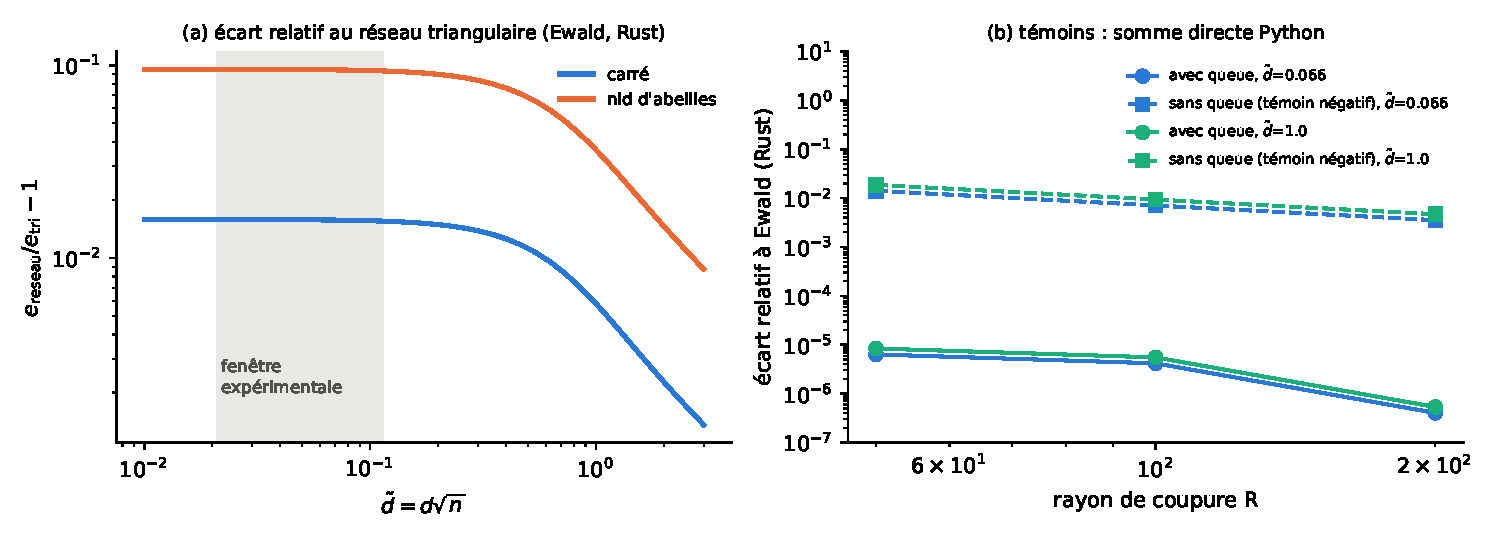
\includegraphics[width=\textwidth]{ch5_U1_dipolar.pdf}
\caption{U1 \tierX. (a) Relative gap of the square and honeycomb lattices to the triangular lattice (exact Ewald
energies, rusty-SUNDIALS), as a function of $\tilde d$. The grey band is the experimental window deduced from
JARVIS-DFT. (b) Controls: a direct sum in Python, \emph{with} the exact uniform tail, converges to the
Ewald value; \emph{without} the tail (negative control), the error stays of order $10^{-2}$.}\label{ch5:fig:U1}
\end{figure}

\paragraph{The result \tierX.} Over the whole grid, both gaps remain positive:
\begin{itemize}
\item $e_\mathrm{square}/e_\mathrm{tri}-1$ decreases from $1.58\times10^{-2}$ to $1.36\times10^{-3}$;
\item the honeycomb gap decreases from $9.53\times10^{-2}$ to $8.75\times10^{-3}$.
\end{itemize}
Converted to energy (unscreened, to be divided by $\varepsilon_r$), the square-minus-triangular gap is
$0.0014$, $0.044$ and $0.224$~meV per exciton at the three densities. These values are interpolated on the grid;
the paper gave $0.223$~meV at the nearest grid point. This is one to five orders of magnitude below the
depth of moiré wells, ``tens to 100~meV''~\cite{ch5:wang}. In the published study, none
of the 21 competitors relaxed by CVODE went below the triangular lattice~\cite{ch2dip}.

\paragraph{The controls.}
\begin{itemize}
\item \emph{Positive.} An independent direct Python sum, plus the exact tail $2\pi/(\sqrt{R^2+\tilde
d^2}+R)$, recovers Rust's Ewald value. The relative deviation is $4.0\times10^{-7}$ at $\tilde d=0.066$ and
$5.3\times10^{-7}$ at $\tilde d=1$, for $R=200$. The Ewald energy is independent of the splitting
parameter $\eta$ to within $9.0\times10^{-15}$.
\item \emph{Negative.} Without the tail, the same sum is off by $3.5\times10^{-3}$ and $4.7\times10^{-3}$ at
$R=200$, and by $1.4\times10^{-2}$ at $R=50$.
\item \emph{Negative.} The script checks that $h_d(d^2)<0$ for $d=0.5$, $1$ and $2$. The square and honeycomb
lattices keep a higher energy at each of the 41 grid points.
\end{itemize}
We also reran, separately, two relaxations of the published study at $\tilde d=0.066$ (command
\texttt{dipolar\_crystal main <dir> 0.066 1 0 1}, about 8~minutes on two cores):
\begin{itemize}
\item the uniform start \texttt{uniform\_00} ends at a relative gap of $1.382373\times10^{-3}$, with 4 defects;
\item the incommensurate box, a negative control, ends at $2.000407\times10^{-3}$, with 8 defects.
\end{itemize}
Both values match the record, digit for digit.

\paragraph{What this does not show.}
\begin{itemize}
\item The model is classical, at zero temperature, with rigid dipoles and no screening: no
Rytova--Keldysh form, no moiré potential, no kinetic energy. In the experimental window, real excitons
form a quantum gas, not a classical crystal~\cite{ch5:wang}.
\item The JARVIS $d$ is a proxy: that of two homogeneous stackings, not that of a heterobilayer. The
dataset fixes the scale of $\tilde d$; it does not test the theorem.
\item No relaxation proves optimality: 21 trials do not cover the infinitely many configurations.
\end{itemize}

% =====================================================================================================
\section{U2 -- Planar Yukawa crystals: dusty plasmas and colloids}\label{ch5:U2}

\paragraph{The question.} In a laboratory dusty plasma, charged microparticles levitate in a plane.
They repel each other through a Coulomb potential screened by the ions, $V(r)=Q^2e^{-r/\lambda_D}/r$. Charged
colloids in suspension behave in the same way. At fixed density, which configuration minimizes the energy?
Hexagonal crystals are observed; can this be proved within this model?

\paragraph{The theorem and its tier.} With $t=r^2$ and $\kappa=\ell/\lambda_D$, where $\ell$ is the length
scale set by the density, $g_\kappa(t)=e^{-\kappa\sqrt t}/\sqrt t$. The human proof \tierC{} proceeds in
three steps:
\begin{itemize}
\item $t\mapsto\sqrt t$ is a Bernstein function and $x\mapsto e^{-\kappa x}$ is completely monotone,
so their composite $e^{-\kappa\sqrt t}$ is completely monotone (this is the CM\,$\circ$\,Bernstein rule of the P3 library, doi:10.5281/zenodo.23653842);
\item $t^{-1/2}$ is completely monotone;
\item a product of two completely monotone functions is again completely monotone (Leibniz rule: every term has the
right sign).
\end{itemize}
Lean checks it \tierA{} (Lean 4.34.1), conditionally on the upstream result:
\begin{leanbox}[: \texttt{formal\_cert/Autoresearch/Yukawa.lean} (statements)]
\begin{lstlisting}[language=Lean]
theorem yukawa_admissible {κ : ℝ} (hκ : 0 < κ) : AdmissiblePotential (g κ)
theorem triangular_yukawa_optimal {κ : ℝ} (hκ : 0 < κ) (C : Set Plane) (hC : LocallyFinite C)
    (hdens : DensityOne C) : latticeEnergy (g κ) ≤ energy (g κ) C
theorem latticeEnergy_yukawa_lt_top {κ : ℝ} (hκ : 0 < κ) : latticeEnergy (g κ) < ⊤
\end{lstlisting}
\end{leanbox}
The module \texttt{YukawaMix.lean} extends the result to every finite mixture $\sum_iw_ie^{-\kappa_ir}/r$ with weights
$w_i\ge0$. The formal negative control is the signed mixture $g_1-2g_2$: it equals $2e^{-1/2}-4e^{-1}\approx-0.2585$
at $t=\tfrac14$, so it is not admissible. The theorem does not apply to it, which does not mean that
optimality fails. Paper: doi:10.5281/zenodo.23646105~\cite{ch2yuk}.

\begin{uniremark}\tierL{} By Bernstein's theorem, a function $g$ on $(0,\infty)$ is completely monotone if and only if
$g(t)=\int_{[0,\infty)}e^{-ts}\,d\mu(s)$ for a positive Borel measure $\mu$~\cite{bernstein,widder}. In this language
the three steps above are closure properties of Laplace transforms of positive measures: a product corresponds to the
convolution of the measures, and composing with a Bernstein function corresponds to subordination. For instance
$e^{-\kappa\sqrt t}$ is the Laplace transform of the one-sided $\tfrac12$-stable (Lévy) density (standard).
\end{uniremark}

\paragraph{The data.} On 2026-10-25, a search of the Hub (\emph{dusty plasma}, \emph{complex plasma},
\emph{colloid}, \emph{yukawa}, \emph{wigner crystal}) found no dataset of grain or colloid
positions~\cite{ch2yuk}. This is an absence observed by search, not a proof. The disordered
initial conditions therefore come from an entirely different field, catalysis:
\begin{itemize}
\item identifier \texttt{colabfit/OC20\_IS2RES\_val\_id}, licence CC-BY-4.0~\cite{ch5:oc20};
\item file \texttt{co/co\_10.parquet}, 142\,986\,687 bytes; its local sha256 equals the Hub's LFS hash at
revision \texttt{6a1dfef12aec878b4cda99edd54b16a6a254e135};
\item adsorbate structures, rotated in 3D, projected onto the plane, rescaled and filtered by a
minimum distance.
\end{itemize}
The script checks the sha256 and finds in the file the OC20 configuration identifiers listed in
\texttt{provenance.json}. These data provide realistic-looking \emph{disorder}, nothing more: molecules
adsorbed on a catalyst have nothing to do with screened charged grains.

\paragraph{The numerical method.} The module \texttt{exact.rs} of \texttt{qf-yukawa-crystal} has three parts:
\begin{itemize}
\item lattice sums of the \emph{untruncated} potential, with a rigorous bound on the tail;
\item an independent Ewald decomposition;
\item a periodic box summing all images within radius $R$, with analytic energy, force and
Hessian.
\end{itemize}
The tail bound relies on Voronoi cells: for decreasing $V$, the tail beyond $R$ is at most
$(\pi/A)\bigl(1+\delta/(R-2\delta)\bigr)e^{-\kappa(R-2\delta)}/\kappa$. The relaxation (\texttt{exact-relax}) uses
CVODE: BDF, Jacobian equal to minus the Hessian, $\mathrm{rtol}=10^{-10}$, $\mathrm{atol}=10^{-12}$ and
force tolerance $10^{-9}$. Each minimum is checked through the spectrum of the Hessian. This computation corrects a
published erratum: an earlier version truncated the potential at $r_c=8$ with a force shift, and this truncated
potential is no longer completely monotone.

\paragraph{The script.} \texttt{code/ch5\_U2\_yukawa.py OUTPUT}:
\begin{enumerate}
\item it copies the initial conditions into a working crate;
\item it runs \texttt{yukawa\_crystal exact-refs}, then \texttt{exact-relax 2 1 0 0}. At $\kappa=2$, this means
three relaxations of about 1 to 2~minutes each on two cores: an OC20 start, a uniform start and an
incommensurate box;
\item it runs the controls and plots \texttt{figures/ch5\_U2\_yukawa.pdf}.
\end{enumerate}
The option \texttt{--skip-relax} rereads the record instead of rerunning the relaxations.

\begin{figure}[ht]\centering
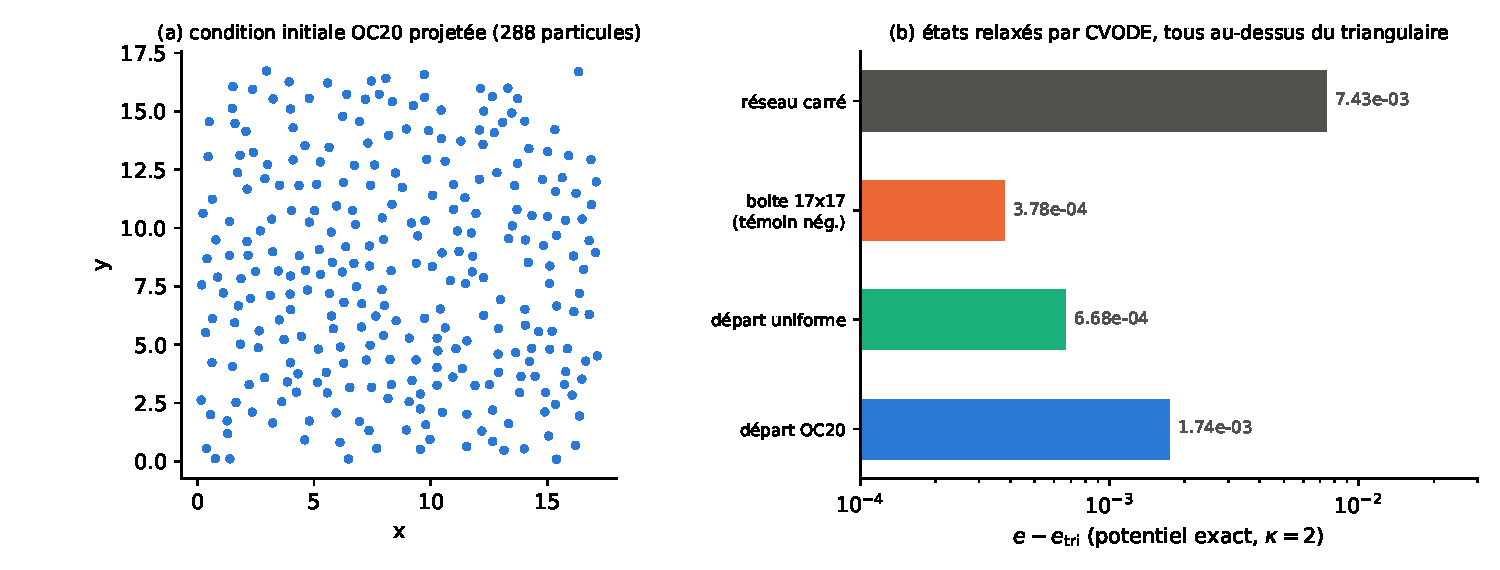
\includegraphics[width=\textwidth]{ch5_U2_yukawa.pdf}
\caption{U2 \tierX. (a) Initial condition drawn from OC20 (288 particles in a box that exactly contains the
triangular lattice). (b) Gap $e-e_\mathrm{tri}$ of the states relaxed by CVODE under the exact potential
($\kappa=2$), to be compared with the gap of the square lattice. No state lies below the triangular
lattice.}\label{ch5:fig:U2}
\end{figure}

\paragraph{The result \tierX.} Energies per particle at density one, in the $\tfrac12\sum$ convention:

\begin{center}\small
\begin{tabular}{lllll}\toprule
$\kappa$ & triangular (exact) & square (exact) & gap & truncated--exact (tri.)\\\midrule
1 & 1.6253213396063 & 1.6348554953172 & $9.534\times10^{-3}$ & $-1.771\times10^{-2}$\\
2 & 0.3935428489324 & 0.4009742487651 & $7.431\times10^{-3}$ & $-9.48\times10^{-6}$\\
\bottomrule\end{tabular}
\end{center}
The tail bound is at most $5.6\times10^{-17}$ ($\kappa=1$, $R=40$) and $1.2\times10^{-16}$ ($\kappa=2$,
$R=20$). The three relaxations at $\kappa=2$ converge, with no negative mode of the Hessian:
\begin{itemize}
\item OC20 start: gap $1.742\times10^{-3}$, 24 defects, 157 CVODE steps;
\item uniform start: gap $6.68\times10^{-4}$, 4 defects;
\item incommensurate $17\times17$ box: gap $3.78\times10^{-4}$, 4 defects.
\end{itemize}
In the full study, none of the 24 stages relaxed under the exact potential went below the triangular
lattice~\cite{ch2yuk}.

\paragraph{The controls.}
\begin{itemize}
\item \emph{Positive.} A direct Python lattice sum recovers Rust's exact values to within
$1.4\times10^{-16}$ in relative terms at most (the required threshold is $10^{-12}$). In addition, the periodic box containing the perfect lattice equals the infinite
sum to within $2.2\times10^{-16}$.
\item \emph{Negative.} The energies truncated at $r_c=8$ miss the exact value by far more than $10^{-9}$. The
$17\times17$ box, which cannot contain the triangular lattice, stays above. The perfect square lattice is a saddle
of the exact potential, with 72 negative modes at $\kappa=2$ and 64 at $\kappa=1$~\cite{ch2yuk}.
\end{itemize}

\paragraph{What this does not show.}
\begin{itemize}
\item The OC20 data contain no plasma physics: they serve only as initial disorder.
\item The potential $K_0(\kappa r)$, the 2D Debye--Hückel Green's function, is not treated. Neither are mixtures with
negative weights, finite temperature or uniqueness.
\item The annealing was not redone with the exact potential.
\end{itemize}

% =====================================================================================================
\section[U3 -- Superfluid helium and the Feynman--Bijl test]{U3 -- Superfluid helium: structure factor and the Feynman--Bijl test}\label{ch5:U3}

\paragraph{The question.} X-ray or neutron diffraction measures the static structure factor $S(k)$
of a liquid. For a weakly interacting Bose gas, Bogoliubov theory predicts
$S_B(k)=\varepsilon_0(k)/\varepsilon_B(k)$, with $\varepsilon_0=\hbar^2k^2/2m$. Can one say, \emph{from
$S(k)$ alone}, that superfluid helium-4 is not a Bogoliubov gas?

\paragraph{The theorem and its tier.} Set $k^*=2mc/\hbar$, where $c$ is the speed of sound. Then
$S_B(k)=k/\sqrt{k^{*2}+k^2}$ and
\[S_B(k)\le\sqrt{\frac{k}{2k^*}},\qquad\text{with equality if and only if }k=k^* .\]
\begin{humanproof}
Both sides are positive; we compare their squares. $S_B^2\le k/2k^*$ is equivalent to
$2k^*k\le k^{*2}+k^2$, that is, to $(k-k^*)^2\ge0$.
\end{humanproof}
\begingroup\sloppy The statement is \tierAs{}, in the QuantumFluids environment (Lean v4.34.0-rc2; no \texttt{leanchecker} replay recorded for this environment), under the name
\lean{sBog_le_sqrt}. Both controls are checked by the kernel: the test fires on the free value $S=1$
for every $0<k<2k^*$ (\lean{free_S_one_violates}), and never fires on $S_B$. The corollary
\lean{not_bogoliubov_of_structure_factor} gives the ``diffraction test'': if a measured $S$ exceeds
$\sqrt{k/2k^*}$, this $S$ is not the structure factor of a Bogoliubov gas with that speed of sound.
The Feynman--Bijl argument relates $S$ to the excitation energy, $\varepsilon(k)\le\hbar^2k^2/(2mS(k))$. Its
single-mode core is formalized in Lean 4.34.1, with the f-sum rule identity taken as a
\emph{hypothesis}. Papers: doi:10.5281/zenodo.23646117~\cite{ch3-bsk} and
doi:10.5281/zenodo.23653846~\cite{ch3-fb}.\par\endgroup

\paragraph{The data (not Hugging Face).} No structure-factor dataset exists on the Hub: the
searches for these two papers found none. We use Table~14.1 of the compilation by Donnelly and
Barenghi~\cite{ch3-db}, in its web edition (assumed, without verification, to reproduce the 1998 table):
\begin{itemize}
\item 99 points with $Q>0$: 49 X-ray points (Robkoff--Hallock) and 50 neutron points (Svensson et al.);
\item temperatures from 1.4 to 4~K, no error bars printed.
\end{itemize}
This is a secondary source at \tierL{}. The extracted file is
\url{papers/prog_superfluid_structure_factor/data/he4_Sk_donnelly_table14_1.csv}. We take
$c=238.3\pm0.1$~m/s~\cite{ch3-godfrin}, whence $k^*=3.00379$~\AA$^{-1}$ (between 3.0025 and 3.0051).

\paragraph{The method.} For each point, the verdict is:
\begin{itemize}
\item \textsc{compatible} if $S\le\sqrt{Q/2k^*}$;
\item \textsc{refuted} if $S-\sqrt{Q/2k^*}>\Delta$;
\item \textsc{undecided} otherwise.
\end{itemize}
The threshold $\Delta=0.082$ is the gap between the maxima of the two datasets in the table. This threshold was fixed after the fact; it
was not preregistered. On the rusty-SUNDIALS side, the module \texttt{linear\_response} of \texttt{qf-gpe2d} gives a
cross-check: one excites the Gross--Pitaevskii ground state ($32\times32$ grid, Strang split step),
measures the frequency of the response, and derives $\varepsilon_B(k)$ and $S(k)$ from it.

\paragraph{The script.} \texttt{code/ch5\_U3\_helium.py OUTPUT [--gpe-json FILE]} applies the test and runs the
controls. If it is given the output of the \texttt{bogoliubov\_dispersion} example of \texttt{qf-gpe2d}, it also plots
the linear response.

\begin{figure}[ht]\centering
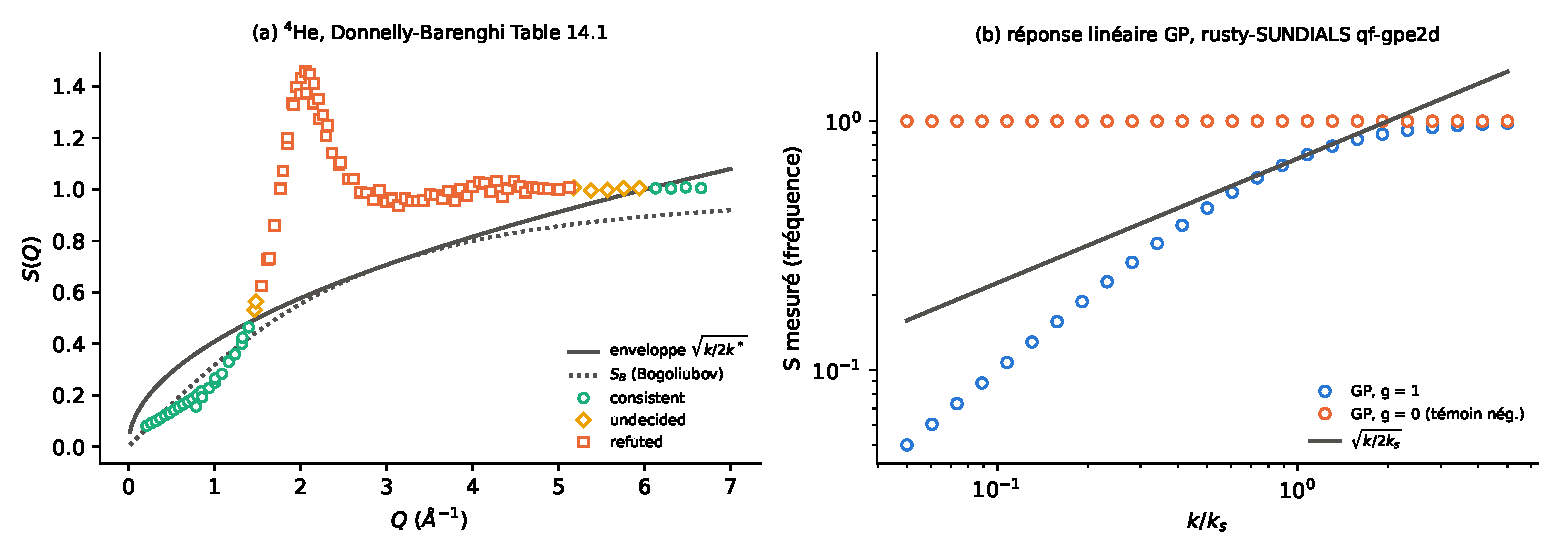
\includegraphics[width=\textwidth]{ch5_U3_helium.pdf}
\caption{U3. (a) $S(Q)$ of helium-4 (Table~14.1, Tier~L) against the envelope $\sqrt{Q/2k^*}$ (solid line) and
$S_B$ (dotted); the colour gives the verdict (arithmetic, Tier~X). (b) Gross--Pitaevskii linear response
computed by rusty-SUNDIALS \tierX{}: measured $S$ for $g=1$ below the envelope, control $g=0$ ($S=1$) above it for
$k<2k_s$.}\label{ch5:fig:U3}
\end{figure}

\paragraph{The result.} Of the 99 points, 29 are compatible, 7 undecided and 63 refuted. The 21 points of the
peak and roton region ($1.7\le Q\le2.4$~\AA$^{-1}$) are all refuted: there $S$ exceeds the envelope by a factor of
1.62 to 2.49. The helium-4 measurements are therefore not the $S$ of a Bogoliubov gas with the same speed of sound. This
textbook result is now a consequence of a checked statement and a published table.

We reran the \texttt{bogoliubov\_dispersion} example (10~min 24~s on one core), and its output is
bit-for-bit identical to the record. In this Gross--Pitaevskii linear response \tierX{}:
\begin{itemize}
\item the frequency measured for $g=1$ recovers $\varepsilon_B$ to within $4.1\times10^{-5}$ in relative terms;
\item the measured $S$ stays below the envelope, since $\max(S/\sqrt{k/2k_s})-1=-1.4\times10^{-3}$;
\item the control $g=0$, a free gas where $S=1$, exceeds the envelope at the 20 wavenumbers of the sweep with
$k<2k_s$.
\end{itemize}

\paragraph{The controls.}
\begin{itemize}
\item \emph{Positive.} $S_B$ fires the test at none of the 99 points.
\item \emph{Negative.} The free value $S=1$ fires it at 95 of the 95 points with $Q<2k^*$.
\end{itemize}
Both controls are also Lean theorems.

\paragraph{What this does not show.}
\begin{itemize}
\item The physical conclusion is conditional \tierC{}: the table was measured between 1.4 and 4~K, not at
$T=0$. We have not quantified how the peak of $S$ varies with temperature.
\item A compatible point is not \emph{confirmed} ``Bogoliubov'': the envelope is only an upper
bound, and at small $k$ it has very little testing power.
\item Beyond the peak, the failure resembles that of the control $S=1$: this is no longer roton physics.
\end{itemize}

% =====================================================================================================
\section[U4 -- Turbulence: enstrophy bound]{U4 -- Turbulence: enstrophy bound in the shell model \texorpdfstring{$\sigma=3$}{sigma=3}}\label{ch5:U4}

\paragraph{The question.} Shell models replace a turbulent velocity field by one complex amplitude
$v_n$ per octave of wavenumbers, $k_n=2^n$, $n=0,\dots,N+1$. Neighbouring shells exchange energy through a
quadratic term. Add a dispersive term $-i\omega_nv_n$ with $\omega_n=Dk_n^3$ (``$\sigma=3$''). Can one
bound the enstrophy $\Omega=\tfrac12\sum k_n^2|v_n|^2$, which measures the small scales, along \emph{every}
trajectory and for \emph{every} truncation $N$?

\paragraph{The theorem and its tier.} The model conserves two quantities:
\begin{itemize}
\item the ``mass'' $S=\sum|v_n|^2=2E$;
\item the invariant $H=\sum2^{-n}\omega_n|v_n|^2+\sum2^{-n}k_n\,\mathrm{Im}(\bar v_n^{\,2}v_{n+1})$, for \emph{every}
real dispersion law.
\end{itemize}
For $\omega_n=Dk_n^3$, the quadratic part of $H$ equals exactly $2D\Omega$. The cubic part $C$ satisfies
$|C|\le S^{3/2}$.
\begin{humanproof}
Write $H_3(0)$ for the value of $H$ at time $0$. Since $H$ is conserved, $2D\Omega(t)=H_3(0)-C(t)$. Hence
$2D\Omega(t)\le H_3(0)+|C(t)|\le H_3(0)+S(t)^{3/2}$. Since $S$ is conserved,
$2D\Omega(t)\le H_3(0)+(2E(0))^{3/2}$.
\end{humanproof}
Lean checks all of this \tierAs{} (Lean v4.34.0-rc2, the project's Mathlib; no \texttt{leanchecker} replay):
\begin{itemize}
\item the rate identity of $H$ along the vector field;
\item the chain rule;
\item the constancy of $H$ and $S$ on $[0,T]$;
\item the bound \lean{enstrophy_bound_along_flow}, for every trajectory on $[0,T]$ and every $N$.
\end{itemize}
\begingroup\sloppy The statement assumes that the trajectory exists and is differentiable at every instant of $[0,T]$: existence is
a \emph{hypothesis}, not a theorem. The level $N$ stays fixed. Paper: doi:10.5281/zenodo.23646111~\cite{ch5:sigma3}.\par\endgroup
\paragraph{The data.} The Well~\cite{ch5:thewell} contains large-scale fluid simulations. We
use:
\begin{itemize}
\item identifier: \url{polymathic-ai/turbulent_radiative_layer_2D};
\item revision \texttt{2ee7756575ff6f90981d0308cbcb6a2ab5995bdc}, licence CC-BY-4.0 according to the card;
\item the file\\ \url{data/test/turbulent_radiative_layer_tcool_0.32.hdf5},\\ sha256 \texttt{06cbd36c\dots f747},
checked by the script.
\end{itemize}
These are Athena++ simulations of the 2D compressible Euler equations with radiative cooling.

The spectrum is built as follows, for four developed snapshots (indices 25, 50, 75 and 100):
\begin{enumerate}
\item take the FFT of the velocity along the periodic axis $x$, without the mode $k_x=0$;
\item average over $y$;
\item sum $k_x\in[2^n,2^{n+1})$ into shell $n=0,\dots,5$.
\end{enumerate}
This step reads the HDF5 file with \texttt{h5py}, which is absent from AutoevolveAI's \texttt{.venv} environment: the script
therefore rereads the file \texttt{well\_amps.txt} that these steps produced. The $\log_2$ slopes of the spectra are
$-2.13$, $-1.56$, $-1.79$ and $-1.81$~\cite{ch5:sigma3}.

\paragraph{The numerical method.} The module \texttt{sigma.rs} of \texttt{qf-shell-cascade} integrates the model with CVODE:
\begin{itemize}
\item BDF, analytic Jacobian, $\mathrm{atol}=10^{-3}\,\mathrm{rtol}$, $D=0.05$;
\item suprema taken at CVODE's internal step points, without interpolation.
\end{itemize}
The program \texttt{sigma3\_study full} runs five blocks in sequence:
\begin{itemize}
\item a positive control, the convergence of conservation with the tolerance;
\item a negative control, a perturbed coupling;
\item a sweep of truncations $n_{\max}\le7$;
\item the comparison $\sigma=2$ versus $\sigma=3$ on data concentrated in the last shell;
\item 24 trajectories initialized from the moduli of The Well, with two draws of random phases and
$n_{\max}=5,6,7$.
\end{itemize}

\paragraph{The script.} \texttt{code/ch5\_U4\_shell.py OUTPUT} runs \texttt{sigma3\_study full} (from 2.5 to 6~minutes
depending on the machine's load), checks the criteria and plots \texttt{figures/ch5\_U4\_shell.pdf}.

\begin{figure}[ht]\centering
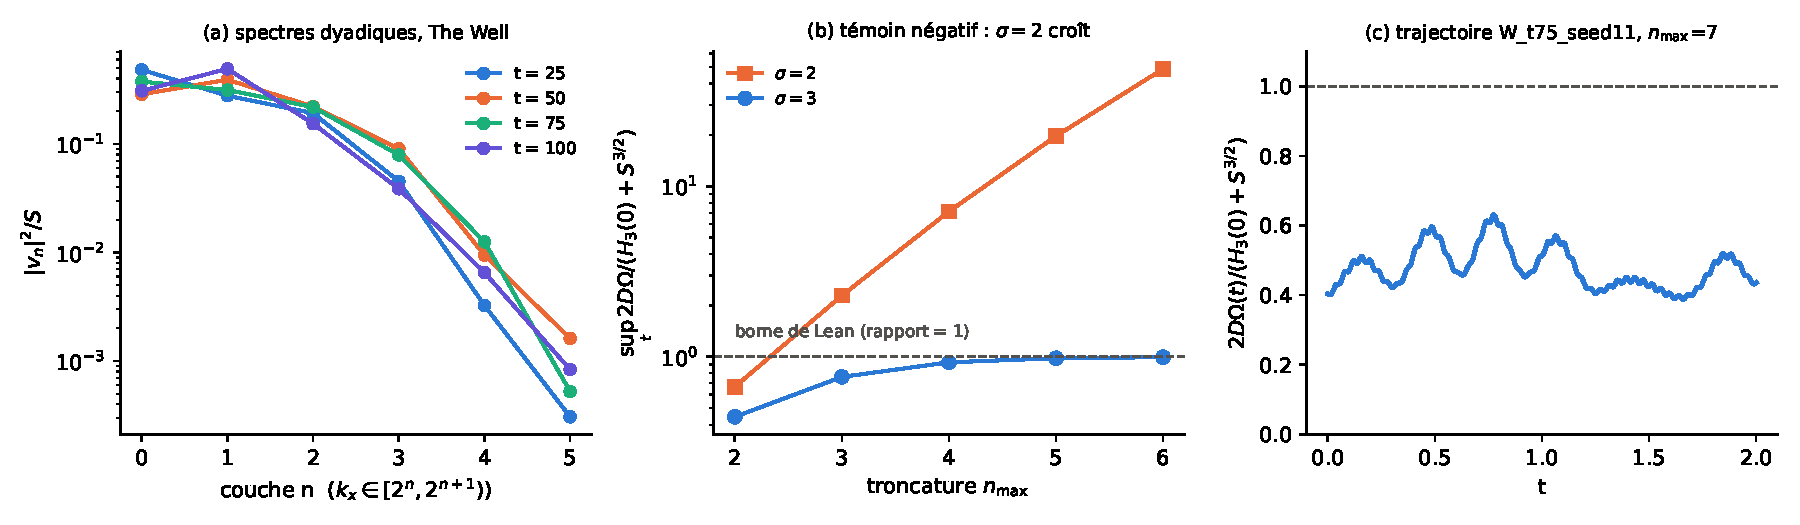
\includegraphics[width=\textwidth]{ch5_U4_shell.pdf}
\caption{U4 \tierX. (a) Dyadic spectra of four snapshots of The Well, normalized to $S=1$. (b) Ratio
$\sup_t2D\Omega/(H_3(0)+S^{3/2})$ on data concentrated in the last shell: it stays below 1 for
$\sigma=3$ and grows with $n_{\max}$ for $\sigma=2$ (negative control). (c) The ratio along the trajectory
initialized from The Well that comes closest to the bound.}\label{ch5:fig:U4}
\end{figure}

\paragraph{The result \tierX.} The 17 $\sigma=3$ trajectories of the sweep and of the comparison all stay below the
bound. The ratio $\sup_t2D\Omega(t)/(H_3(0)+S(0)^{3/2})$ is at most 0.995; this maximum is reached on data
concentrated in the last shell, where the ratio tends to 1 as $n_{\max}$ grows (0.444, 0.762, 0.928, 0.981
and 0.995 for $n_{\max}=2,\dots,6$). The 24 trajectories initialized from The Well also stay below the bound, with
a ratio of at most 0.631. Their relative drifts are at most $2.4\times10^{-8}$ on $S$ and $1.2\times10^{-6}$
on $H$. The recomputed file \texttt{sigma3\_study.json} is identical to the record of
the paper~\cite{ch5:sigma3}, up to run times.

\paragraph{The controls.}
\begin{itemize}
\item \emph{Positive.} With the true coupling, the drift of $H$ decreases with the tolerance. For $n_{\max}=4$, it
is $2.6\times10^{-5}$, $8.6\times10^{-7}$ and then $1.9\times10^{-8}$ for
$\mathrm{rtol}=10^{-6},10^{-8},10^{-10}$.
\item \emph{Negative.} If the coupling leaving shell~1 is perturbed by $10^{-2}$, the drift of $H$ stays
stuck near $2.3\times10^{-3}$ ($n_{\max}=4$) and $5.4\times10^{-3}$ ($n_{\max}=6$), whatever the
tolerance. Conservation therefore comes from the structure of the model, not from the accuracy of the solver.
\item \emph{Negative.} For $\sigma=2$, the same inequality has no proof, and the ratio is 0.667, 2.29,
7.11, 19.7 and then 48.8 for $n_{\max}=2,\dots,6$. It exceeds 1 from $n_{\max}=3$ on and grows faster than an
exponential of ratio 2 over this range (Figure~\ref{ch5:fig:U4}b).
\end{itemize}

\paragraph{What this does not show.}
\begin{itemize}
\item The Well data give a realistic spectral shape, and nothing else. The flow is compressible
and cooled; it does not conserve energy. The spectrum is one-dimensional and carries no phases (they are
drawn at random).
\item Over $T=2$, the upper shells, initially empty, barely fill up. These trajectories therefore do not probe
the dependence on $N$.
\item There is no statement for infinitely many shells. Uniformity in $N$ requires initial data whose
$\Omega(0)$ and $S(0)$ are bounded uniformly in $N$ (a Tier C corollary).
\item BDF damping makes $S$ drift downwards. The observed margins far exceed these drifts,
but the simulation does not replace the theorem.
\end{itemize}

% =====================================================================================================
\section{U5 -- Genetics: fixation of a mutation}\label{ch5:U5}

\paragraph{The question.} A population has $N$ individuals, $i$ of whom carry a mutation of relative
fitness $r$. What is the probability that the mutation eventually takes over the whole population
(\emph{fixation})? And what becomes of this probability when the population lives on a graph?

\paragraph{The Moran model.} At each step, one individual is chosen to reproduce with probability
proportional to its fitness, and one individual drawn uniformly at random dies. The number of mutants is a
birth--death chain on $\{0,\dots,N\}$. Its up and down probabilities are
\[p_i=\frac{ri}{ri+N-i}\cdot\frac{N-i}{N},\qquad q_i=\frac{N-i}{ri+N-i}\cdot\frac iN,\qquad\text{hence } p_i=r\,q_i .\]

\paragraph{The theorem and its tier.} Write $\varphi_i$ for the fixation probability starting from $i$ mutants. The
first-step equation gives $p_i(\varphi_{i+1}-\varphi_i)=q_i(\varphi_i-\varphi_{i-1})$, with $\varphi_0=0$ and
$\varphi_N=1$.
\begin{humanproof}[Human proof (formula)]
Set $\delta_i=\varphi_{i+1}-\varphi_i$. The equation gives $\delta_i=\delta_{i-1}/r$, hence $\delta_i=r^{-i}\delta_0$
and $\varphi_i=\delta_0S_i$, where $S_i=\sum_{k<i}r^{-k}$. The condition $\varphi_N=1$ fixes
$\delta_0=1/S_N$. For $r\ne1$, we obtain
\[\varphi_i=\frac{S_i}{S_N}=\frac{1-r^{-i}}{1-r^{-N}} .\]
For $r=1$, we obtain $\varphi_i=i/N$.
\end{humanproof}
Programme P7 checks more \tierA{} (Lean 4.34.1). It proves the \emph{absorption limit},
$P^n(i,N)\to(1-r^{-i})/(1-r^{-N})$, and uniqueness: every function that is harmonic in the interior with values $0$ and
$1$ on the boundary equals $\varphi$. Programme N4 proves the isothermal theorem (birth--death): on a
strongly connected graph whose replacement matrix is doubly stochastic, fixation follows the same law.
\begin{leanbox}[: \texttt{PopGen/MoranFixation.lean} and \texttt{EvoGraph/BirthDeath.lean} (statements)]
\begin{lstlisting}[language=Lean]
theorem moran_fixation_limit_closed {N : ℕ} {r : ℝ} (hN : 0 < N) (hr : 0 < r) (hr1 : r ≠ 1)
    (i : Fin (N + 1)) :
    Tendsto (fun n => kPow (moranP N r) n i (Fin.last N)) atTop
      (𝓝 ((1 - r⁻¹ ^ (i : ℕ)) / (1 - r⁻¹ ^ N)))
theorem moran_fixation_unique {N : ℕ} {r : ℝ} (hN : 0 < N) (hr : 0 < r) {g : Fin (N + 1) → ℝ}
    (hg : InteriorHarmonic (moranP N r) g) (g0 : g 0 = 0) (g1 : g (Fin.last N) = 1) :
    ∀ i, g i = moranFix N r i
theorem isothermal_fixation {W : Fin n → Fin n → ℝ} {r : ℝ} (hn : 0 < n) (hr : 0 < r)
    (hW : Isothermal W) (hsc : StronglyConnected W) (S : Finset (Fin n)) :
    Tendsto (fun t => sPow (bdK (fun _ => 1) W r) t S univ) atTop (𝓝 (moranFix n r S.card))
\end{lstlisting}
\end{leanbox}
The general absorption theorem of P7 and the single-mutant version of the isothermal theorem reappear under
the names \lean{KAL} and \lean{ILENE} in Section~\ref{ch5:acronymes}.

\begin{uniremark}\tierL{} For a finite absorbing Markov chain, the absorption probabilities form the unique bounded
solution of the first-step equations that is harmonic at the transient states and takes the prescribed boundary values;
equivalently, if $h$ is such a solution then $h(X_n)$ is a bounded martingale and the optional stopping theorem at the
absorption time gives $h(i)=\mathbb P_i(\text{absorption at }N)$~\cite{app:norris,app:williams}.
\end{uniremark}

The number of mutants on a graph is \emph{not} a Markov chain in general. On the 4-cycle, the one-step up
probability depends on the configuration, $1/3$ versus $2/3$ at $r=2$. What is true, and proved, is the bias
\emph{per configuration} $P^+=r\,P^-$. On the star with $n=3$ nodes, which is not isothermal, the limits are
$5/12$, $2/3$ and $7/12$, against $4/7$ for Moran. Papers: doi:10.5281/zenodo.23653850~\cite{ch4:P7} and
doi:10.5281/zenodo.23660071~\cite{ch4:N4}.

\paragraph{The data: what they illustrate, and what they do not estimate.} The author's Genetic repository
uses the datasets \texttt{katarinagresova/Genomic\_Benchmarks\_*}~\cite{ch5:gb}. We take one of them:
\begin{itemize}
\item identifier \url{katarinagresova/Genomic_Benchmarks_demo_coding_vs_intergenomic_seqs}, revision
\texttt{85458172cab6cffad46cb172e64ca94780506ed6};
\item the test split, \url{data/test-00000-of-00001-6fccc31405110e30.parquet}, 2\,456\,511 bytes, sha256
\texttt{dfe13715\dots 9afe}.
\end{itemize}
The card states \emph{no} licence and does not say what the labels 0 and 1 mean. We
reproduce only aggregate statistics, and the licence of the upstream package has not been checked.

The script counts 25\,000 sequences, 12\,500 per label, all of length 200, with no symbol other than A, C, G and T.
The GC fraction is 0.5381 for label~0 and 0.4004 for label~1 (Figure~\ref{ch5:fig:U5}c).

This is what sequence data look like: a point mutation is the replacement of one letter.
\textbf{But this dataset estimates no fitness $r$}, and nothing in this chapter derives one from it. The values of $r$
used below (0.8, 1, 1.2, 1.5 and 2) are \emph{chosen}, not measured.

\paragraph{The numerical method.} The crate \texttt{qf-popgen} writes the absorbing chain as a linear
differential equation, $\dot\pi=\pi(P-I)$: this is the forward Kolmogorov equation of the uniformized chain. It
integrates it with CVODE (BDF, exact Jacobian, $\mathrm{rtol}=10^{-11}$, $\mathrm{atol}=10^{-15}$). An
\emph{absorption certificate} rejects any doubtful run, in a ``fail-closed'' spirit (rejecting by default): a run is
accepted only if five conditions hold:
\begin{itemize}
\item the kernel is stochastic and absorbing;
\item the total mass is conserved;
\item no component becomes negative;
\item the interior mass has dropped below $10^{-9}$;
\item the mass at $N$ equals the target to within $10^{-8}$.
\end{itemize}
The passage from the differential equation to the $n$-step kernel (a Poisson mixture) is not formalized.

Finally, \textbf{LeanFlow} certifies a computed number. Its function \texttt{lean.certify} accepts a claim about
rational enclosures and translates it into a statement about integers. The tactic \texttt{decide\_kernel}
(\lean{decide +kernel}) has this statement decided by the kernel, with no extra axiom. LeanFlow then audits
\texttt{\#print axioms}, and an exact Python oracle must return the same verdict.

\paragraph{The script.} \texttt{code/ch5\_U5\_fixation.py OUTPUT}:
\begin{enumerate}
\item it downloads the file at the pinned revision, checks its digest and computes the statistics;
\item it runs \texttt{fixation\_ode};
\item it compares the CVODE values with the exact fractions;
\item it submits five claims to LeanFlow (Lean 4.34.1, core only);
\item it plots \texttt{figures/ch5\_U5\_fixation.pdf}.
\end{enumerate}
It takes about twenty seconds.

\begin{figure}[ht]\centering
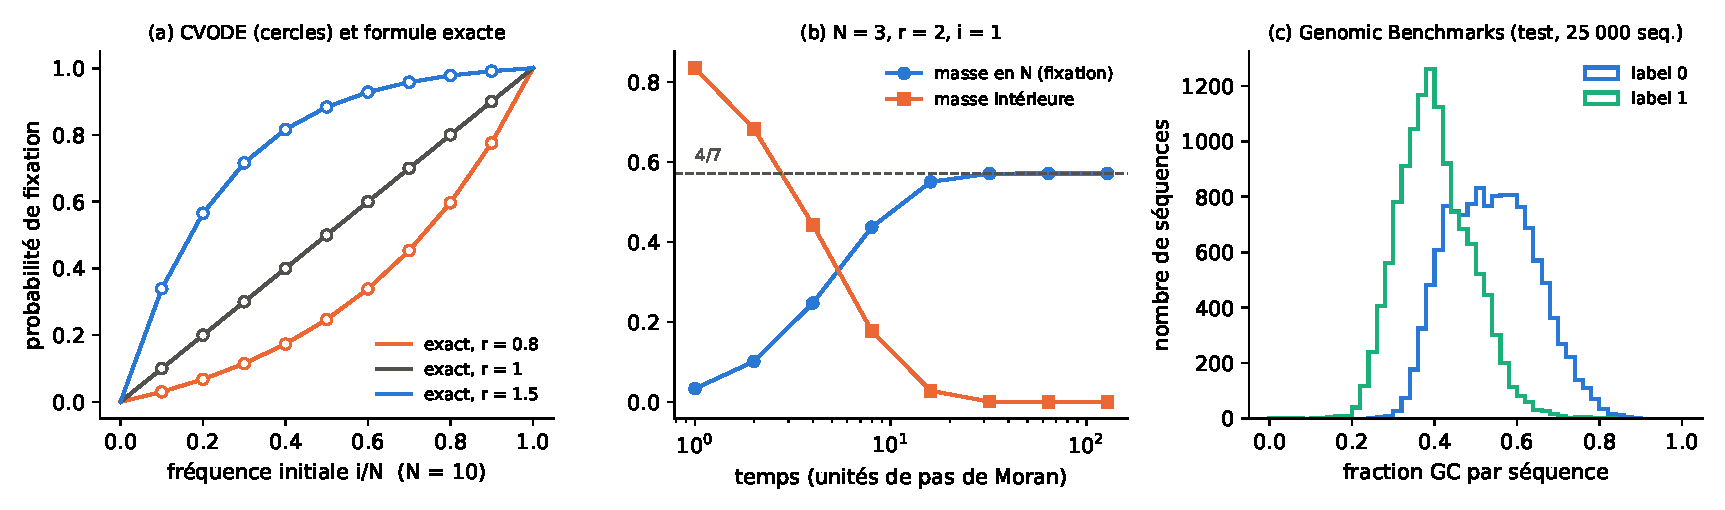
\includegraphics[width=\textwidth]{ch5_U5_fixation.pdf}
\caption{U5. (a) Fixation probability for $N=10$: CVODE (circles, \tierX) and exact formula (lines), for
$r=0.8$, $1$ and $1.5$. (b) CVODE trajectory for $N=3$, $r=2$, $i=1$: the mass absorbed at $N$ tends to
$4/7$, the interior mass dies out. (c) GC fraction of the 25\,000 test sequences of Genomic Benchmarks; this
dataset illustrates sequence data and estimates no fitness.}\label{ch5:fig:U5}
\end{figure}

\paragraph{The result.} \texttt{fixation\_ode} produces 115 rows: 106 accepted runs and 9 negative controls
rejected, without a single exception. Over the accepted Moran runs, the maximal deviation between CVODE and the exact
fraction $S_i/S_N$ is $3.1\times10^{-10}$ \tierX.

For $N=3$, $r=2$, $i=1$, CVODE gives $0.5714285714284759$, a deviation of $9.55\times10^{-14}$ from $4/7$.
LeanFlow then certifies two claims \tierA{} (on the arithmetic statement only, empty axiom list; each claim is split by LeanFlow into elementary propositions):
\begin{itemize}
\item \emph{proximity}: $4/7-10^{-11}<0.5714285714284759<4/7+10^{-11}$;
\item \emph{harmonicity}: the vector $(0,\tfrac47,\tfrac67,1)$ satisfies exactly the first-step equations of the
chain $N=3$, $r=2$, with $p_1=\tfrac13$, $q_1=\tfrac16$, $p_2=\tfrac4{15}$ and $q_2=\tfrac2{15}$.
\end{itemize}
Here is one of the four generated propositions, as the kernel decided it:
\begin{lstlisting}[language=Lean]
-- harmonic at i=1
theorem cert_2 : (0 : Int) < ((((3 : Int) * (7 : Int)) * ((6 : Int) * (1 : Int))) * ((2 : Int) * (7 : Int))) ∧ ((((1 : Int) * (6 : Int)) * ((6 : Int) * (1 : Int)) + ((1 : Int) * (0 : Int)) * ((3 : Int) * (7 : Int))) * ((2 : Int) * (7 : Int)) + ((-1 : Int) * (4 : Int)) * (((3 : Int) * (7 : Int)) * ((6 : Int) * (1 : Int)))) * (1 : Int) = (0 : Int) * ((((3 : Int) * (7 : Int)) * ((6 : Int) * (1 : Int))) * ((2 : Int) * (7 : Int))) := by decide +kernel
\end{lstlisting}
LeanFlow audits only \texttt{\#print axioms}, which can be fooled; we therefore completed the
Tier~A gate for these two certificates. The two generated sources were recompiled to \texttt{.olean} with Lean
4.34.1 and replayed by \texttt{leanchecker}: exit code~0 for both. The control for this step, a missing
module, exits with code~1. A search for \texttt{skipKernelTC}, \texttt{addDecl}, \texttt{native\_decide} and
\texttt{implemented\_by} in the two sources finds nothing.

Combined with \lean{moran_fixation_unique}, harmonicity says that $4/7$ \emph{is} the fixation probability in this case.
This link is a human argument \tierC{}: it identifies LeanFlow's whole statement with the definitions
\lean{moranP} of P7. P7 in fact already contains \lean{cert_N3_r2_i1}, a hand-written Lean certificate for the same
value.

\paragraph{The controls.}
\begin{itemize}
\item \emph{Negative, LeanFlow.} Three false claims are \emph{rejected} (\texttt{false-statement}), and
\texttt{\#print axioms} reports \lean{sorryAx} for them:
\begin{itemize}
\item the neutral value $1/3$ in place of $4/7$;
\item a tolerance that is too tight, $10^{-14}$, smaller than the actual error of $9.55\times10^{-14}$;
\item the neutral vector $(0,\tfrac13,\tfrac23,1)$, which violates both interior equations.
\end{itemize}
\item \emph{Negative, CVODE.} Nine controls are rejected, each for the intended reason:
\begin{itemize}
\item the formula with inverted exponent and the neutral value $i/N$ under selection (\texttt{ValueMismatch}, three
each);
\item the identity kernel, which never absorbs, and a horizon that is too short (\texttt{NotAbsorbed});
\item a row whose sum is $1.001$ (\texttt{InvalidKernel}).
\end{itemize}
\item \emph{Positive.} The cases $N=2$ and $N=3$ at $r=2$ recover $2/3$, $4/7$ and $6/7$, and the neutral case recovers $i/N$.
\end{itemize}

\paragraph{What this does not show.}
\begin{itemize}
\item The Genomic Benchmarks dataset estimates neither $r$, nor $N$, nor any population-dynamics parameter. Its role
is pedagogical.
\item The LeanFlow certificate concerns the arithmetic of the stated numbers, not the correctness of CVODE.
\item The Moran model assumes a constant size, a single locus and a constant $r$. The isothermal theorem is
proved in the ``sufficient'' direction only, for the birth--death rule; the converse and the
death--birth rule are not proved.
\end{itemize}

% =====================================================================================================
\section{Summary: what the five cases teach}\label{ch5:bilan}

\begin{table}[ht]\centering\small
\caption{Controls run for this chapter (script outputs of 2026-10-26).}\label{ch5:tab:temoins}
\begin{tabular}{p{1.4cm}p{6.2cm}p{6.2cm}}\toprule
case & positive control (must succeed) & negative control (must fail)\\\midrule
U1 & direct Python sum $+$ exact tail: $4\times10^{-7}$ from the Rust Ewald value ($R=200$) &
without the tail: error $3.5\times10^{-3}$; $h_d(d^2)<0$; incommensurate box above\\
U2 & direct Python sum: $\le1.4\times10^{-16}$ from Rust &
energies truncated at $r_c=8$: error $\ge9.4\times10^{-6}$; $17\times17$ box above\\
U3 & $S_B$ never fires the test (0 of 99); GP $g=1$ below the envelope &
$S=1$ fires it (95 of 95); GP $g=0$ above (20 of 20)\\
U4 & drift of $H$ divided by $\approx10^3$ when rtol goes from $10^{-6}$ to $10^{-10}$ &
perturbed coupling: drift stuck near $2$--$5\times10^{-3}$; $\sigma=2$ exceeds the bound\\
U5 & 106 accepted runs; two LeanFlow certificates \texttt{ok} &
9 CVODE controls rejected; 3 LeanFlow claims rejected\\
\bottomrule\end{tabular}
\end{table}

Three lessons emerge from the five cases.

\paragraph{Real data are not a proof.} None of the five datasets tests a Tier~A theorem.
Each has a more modest, but real, role:
\begin{itemize}
\item JARVIS-DFT fixes the physical scale $\tilde d$;
\item OC20 provides initial disorder;
\item the Donnelly and Barenghi table \emph{refutes} a modelling hypothesis (``helium is a
Bogoliubov gas'');
\item The Well gives a spectral shape;
\item Genomic Benchmarks shows what a sequence looks like.
\end{itemize}
Case U3 is the only one where the data say something physical. Even then it is \emph{thanks to} the theorem: the
refutation is meaningful only because the envelope is proved.

\paragraph{Disagreement is more instructive than agreement.} Agreement between CVODE and an exact formula, to within
$3\times10^{-10}$ (U5) or $10^{-16}$ (U2), is reassuring about the code, but it says nothing about the model. It is
the negative controls that give the positive controls their value:
\begin{itemize}
\item in U2, an innocent truncation changes the energy by $1.8\times10^{-2}$, twice the gap between square and
triangular;
\item in U4, a coupling perturbed by 1\% destroys a conservation law that no accuracy restores;
\item in U5, a tolerance of $10^{-14}$ is rejected because the actual error is $9.55\times10^{-14}$.
\end{itemize}

\paragraph{Each tool has its scope.} The three tools share the work:
\begin{itemize}
\item Lean checks statements about definitions;
\item rusty-SUNDIALS computes in floating point;
\item LeanFlow bridges the two, by certifying that a \emph{stated} number satisfies an exact relation.
\end{itemize}
None of the three says that the model describes nature. Each section therefore ends with ``what this does not
show'', and that heading counts as much as the result.

% =====================================================================================================
\section{The hidden acronyms}\label{ch5:acronymes}

A few theorems of this book carry, in the Lean code, a second name made of initials. These names
prove nothing new: they are re-exports of results already checked by the kernel, each accompanied
by a backronym in its documentation. They are collected in
the file \texttt{Acronymes.lean} of \texttt{formal\_cert/Programmes/}, listed below.

\IfFileExists{acronymes_listing.tex}{% Generated from formal_cert/Programmes/Famille/Acronymes.lean (verbatim copy); do not edit by hand.
% Requires the book preamble (listings + \lstdefinelanguage{Lean} in main.tex).
\begin{lstlisting}[language=Lean,literate={ℝ}{{$\mathbb{R}$}}1 {ℤ}{{$\mathbb{Z}$}}1 {ℕ}{{$\mathbb{N}$}}1 {≤}{{$\le$}}1 {≥}{{$\ge$}}1 {≠}{{$\ne$}}1
  {→}{{$\to$}}1 {↔}{{$\leftrightarrow$}}1 {∀}{{$\forall$}}1 {∃}{{$\exists$}}1 {∧}{{$\wedge$}}1 {∨}{{$\vee$}}1
  {¬}{{$\neg$}}1 {⊤}{{$\top$}}1 {∈}{{$\in$}}1 {∉}{{$\notin$}}1 {∩}{{$\cap$}}1 {⁻¹}{{$^{-1}$}}1 {√}{{$\surd$}}1
  {π}{{$\pi$}}1 {ρ}{{$\rho$}}1 {κ}{{$\kappa$}}1 {α}{{$\alpha$}}1 {δ}{{$\delta$}}1 {ε}{{$\varepsilon$}}1 {σ}{{$\sigma$}}1
  {•}{{$\bullet$}}1 {∑}{{$\sum$}}1 {²}{{$^2$}}1 {₀}{{$_0$}}1 {₁}{{$_1$}}1 {₂}{{$_2$}}1 {‖}{{$\|$}}1 {⟨}{{$\langle$}}1 {⟩}{{$\rangle$}}1
  {𝓝}{{$\mathcal{N}$}}1 {∞}{{$\infty$}}1 {≥}{{$\ge$}}1 {×}{{$\times$}}1 {·}{{$\cdot$}}1 {∘}{{$\circ$}}1 {∖}{{$\setminus$}}1
  {ψ}{{$\psi$}}1 {φ}{{$\varphi$}}1 {λ}{{$\lambda$}}1 {μ}{{$\mu$}}1 {θ}{{$\theta$}}1 {Λ}{{$\Lambda$}}1 {∂}{{$\partial$}}1
  {—}{{---}}1 {–}{{--}}1 {é}{{\'e}}1 {ö}{{\"o}}1 {’}{{'}}1 {∫}{{$\int$}}1 {ι}{{$\iota$}}1]
import Triangular.AnyDensity
import Programmes.PopGen.Absorption
import Programmes.EvoGraph.BirthDeath
import Autoresearch.KeldyshCM
import Programmes.PopGen.Price

/-!
# Acronymes : cinq ré-exportations sous des noms courts

Each theorem below is a **re-export** of a result that is already kernel-checked elsewhere in
`formal_cert/`. The statement is copied verbatim from the source theorem and the proof is the source
theorem applied to its arguments; nothing new is proved here. The `example`s after each theorem check,
by `rfl`, that the re-exported constant has exactly the type of its source (same statement, not a
weaker or stronger one).

Each name is an acronym; its docstring gives the backronym.

| name      | source                                                     |
|-----------|------------------------------------------------------------|
| `ALIX`    | `TriangularDensity.triangular_optimal_any_density`         |
| `KAL`     | `ProgPopGen.fixation_limit`                                |
| `ILENE`   | `EvoGraph.isothermal_fixation_single`                      |
| `ALEXIS`  | `AutoresearchKeldysh.laplace_admissible`                   |
| `AURELIA` | `ProgPopGen.Price.fisher_haploid_nondecreasing`            |

`ALIX` rests on upstream openai/math `universal_energy_minimum` (AI-generated, not peer reviewed);
everything is conditional on the fidelity of the definitions it uses.
-/

namespace Acronymes

section Lattice

open OAI.AtomicTriangular TriangularDensity Filter Topology Set
open scoped Pointwise

/-- **A** **L**attice **I**s e**X**tremal.

At every density `ρ > 0` the rescaled triangular lattice `ρ^{-1/2} A` is locally finite, has density
`ρ`, and its lower energy is `≤` that of every locally finite density-`ρ` configuration, for every
admissible (completely monotone in `r²`) potential `h`. Re-export of
`TriangularDensity.triangular_optimal_any_density` (conditional on upstream). -/
theorem ALIX (h : ℝ → ℝ) (hh : AdmissiblePotential h) {ρ : ℝ} (hρ : 0 < ρ) :
    LocallyFinite ((Real.sqrt ρ)⁻¹ • A) ∧ DensityRho ρ ((Real.sqrt ρ)⁻¹ • A) ∧
      ∀ C : Set Plane, LocallyFinite C → DensityRho ρ C → energy h ((Real.sqrt ρ)⁻¹ • A) ≤ energy h C :=
  triangular_optimal_any_density h hh hρ

example : @ALIX = @triangular_optimal_any_density := rfl

end Lattice

section Absorption

open Filter Topology ProgPopGen

/-- **K**olmogorov **A**bsorption **L**imit.

For a stochastic kernel on `{0,...,N}` with absorbing ends, whose `n`-step kernel is the
Chapman–Kolmogorov power `kPow P n`: if `h` is interior-harmonic with `h 0 = 0`, `h N = 1` and the
one-step variance of `h` is positive at every interior state, then `P^n(i,N) → h i` and
`P^n(i,0) → 1 - h i`. Re-export of `ProgPopGen.fixation_limit`. -/
theorem KAL {N : ℕ} {P : Fin (N + 1) → Fin (N + 1) → ℝ} (hP : AbsorbingChain P) (hN : 0 < N)
    {h : Fin (N + 1) → ℝ} (hh : InteriorHarmonic P h) (h0 : h 0 = 0) (h1 : h (Fin.last N) = 1)
    (hvar : ∀ k : Fin (N + 1), 0 < (k : ℕ) → (k : ℕ) < N → 0 < ∑ j, P k j * (h j - h k) ^ 2)
    (i : Fin (N + 1)) :
    Tendsto (fun n => kPow P n i (Fin.last N)) atTop (𝓝 (h i)) ∧
    Tendsto (fun n => kPow P n i 0) atTop (𝓝 (1 - h i)) :=
  fixation_limit hP hN hh h0 h1 hvar i

example : @KAL = @fixation_limit := rfl

end Absorption

section Isothermal

open Finset Filter Topology EvoGraph

/-- **I**sothermal **L**aw: **E**very **N**ode **E**quivalent.

Birth–death updating with uniform selection on a strongly connected isothermal graph (`W` doubly
stochastic): a single mutant of fitness `r ≠ 1` placed at *any* node `v` fixes with limiting
probability `(1 - r⁻¹)/(1 - r^(-n))`, the same for every node and equal to Moran's value.
Re-export of `EvoGraph.isothermal_fixation_single`. -/
theorem ILENE {n : ℕ} {W : Fin n → Fin n → ℝ} {r : ℝ} (hn : 0 < n) (hr : 0 < r)
    (hr1 : r ≠ 1) (hW : Isothermal W) (hsc : StronglyConnected W) (v : Fin n) :
    Tendsto (fun t => sPow (bdK (fun _ => 1) W r) t {v} univ) atTop
      (𝓝 ((1 - r⁻¹) / (1 - r⁻¹ ^ n))) :=
  isothermal_fixation_single hn hr hr1 hW hsc v

example : @ILENE = @isothermal_fixation_single := rfl

end Isothermal

section Laplace

open MeasureTheory OAI.AtomicTriangular AutoresearchKeldysh

/-- **A**veraged **L**aplace **EX**ponentials **I**nherit **S**igns.

A positive mixture of decaying exponentials `fun t => ∫ e^{-t k(x)} m(x) dμ(x)` (with `k, m ≥ 0` and all
moments `∫ k^n e^{-c k} m dμ` finite for `c > 0`) is `AdmissiblePotential`: `C^∞` on `(0, ∞)`,
nonnegative, with alternating signs `(-1)^r g^{(r)} ≥ 0`, each exponential's signs passing to the
average. Re-export of `AutoresearchKeldysh.laplace_admissible`. -/
theorem ALEXIS {α : Type*} [MeasurableSpace α] {μ : Measure α} {k m : α → ℝ}
    (h : MixtureData μ k m) :
    AdmissiblePotential (fun t => ∫ x, Real.exp (-(t * k x)) * m x ∂μ) :=
  laplace_admissible h

example : @ALEXIS.{0} = @laplace_admissible.{0} := rfl

end Laplace

section Fisher

open ProgPopGen.Price

/-- **A**verage **U**nder **R**eplication: **E**volution **L**ifts **I**t, **A**lways.

Haploid selection with constant type fitnesses and no transmission bias, nonnegative abundances,
positive total abundance and positive mean fitness: the mean fitness does not decrease,
`wbar ≤ wbar'`. This is a special case of Fisher's fundamental theorem (haploid types, constant
fitnesses, no transmission bias), obtained from the exact identity `wbar' - wbar = Var(w)/wbar`
derived from the Price equation. Re-export of `ProgPopGen.Price.fisher_haploid_nondecreasing`. -/
theorem AURELIA {ι : Type*} (s : Finset ι) (n w : ι → ℝ)
    (hn : ∀ i ∈ s, 0 ≤ n i) (hN : 0 < ∑ i ∈ s, n i) (hW : 0 < ∑ i ∈ s, n i * w i) :
    wmean s n w ≤ wbarNext s n w :=
  fisher_haploid_nondecreasing s n w hn hN hW

example : @AURELIA.{0} = @fisher_haploid_nondecreasing.{0} := rfl

end Fisher

end Acronymes

#print axioms Acronymes.ALIX
#print axioms Acronymes.KAL
#print axioms Acronymes.ILENE
#print axioms Acronymes.ALEXIS
#print axioms Acronymes.AURELIA
\end{lstlisting}
}{}

% =====================================================================================================
\section{Exercises}\label{ch5:exercices}
Exercises marked (S) require running a script; allow at most two cores, for example with
\texttt{taskset -c 6,7}.

\begin{exercise}[U1, computation]\label{ch5:ex:hd}
\begin{enumerate}
\item Show that $h_d(t)=t^{-1/2}-2(t+d^2)^{-1/2}$ satisfies $h_d(d^2)=(1-\sqrt2)/d$. Deduce that $h_d$ is
not completely monotone.
\item With $a=t^{-1/2}$ and $b=(t+d^2)^{-1/2}$, establish $(a-b)(a+b)=d^2a^2b^2$, and then $g_d(t)\le d^2t^{-3/2}$.
Why does this inequality guarantee that \lean{latticeEnergy (g d)} is finite?
\end{enumerate}
\end{exercise}

\begin{exercise}[U1, (S)]\label{ch5:ex:U1}
Run \texttt{ch5\_U1\_dipolar.py}.
\begin{enumerate}
\item Check in the JSON that $\tilde d=0.0660$ at $n=10^{12}$~cm$^{-2}$.
\item Add the density $n=5\times10^{11}$~cm$^{-2}$ and give the square-minus-triangular gap in meV for
$\varepsilon_r=4$.
\item Replace the exact tail by $0$ for $R=400$. Is the error halved compared with $R=200$?
Explain this with the tail formula.
\end{enumerate}
\end{exercise}

\begin{exercise}[U2, computation]\label{ch5:ex:U2a}
Check by hand that $g_1-2g_2$ is negative at $t=\tfrac14$. Then show that a mixture
$\sum_iw_ie^{-\kappa_i\sqrt t}/\sqrt t$ with positive weights is completely monotone, taking the single-term case
for granted.
\end{exercise}

\begin{exercise}[U2, (S)]\label{ch5:ex:U2b}
In \texttt{exact\_refs.jsonl}, produced by the script, the rows \texttt{"kind":"sweep"} give the error of the
truncated energies (\texttt{sf\_err}) as a function of $r_c$.
\begin{enumerate}
\item Plot $|\texttt{sf\_err}|$ at $\kappa=1$. From which $r_c$ on does it become smaller than the square-minus-triangular
gap, $9.5\times10^{-3}$?
\item Compare with the Voronoi tail bound.
\end{enumerate}
\end{exercise}

\begin{exercise}[U3, proof]\label{ch5:ex:U3a}
\begin{enumerate}
\item Show that $S_B(k)=\varepsilon_0/\varepsilon_B$ with $\varepsilon_B=\sqrt{\varepsilon_0(\varepsilon_0+2gn)}$
can be written $k/\sqrt{k^{*2}+k^2}$, where $k^*=2mc/\hbar$ and $mc^2=gn$.
\item Establish the envelope $S_B\le\sqrt{k/2k^*}$ and its equality case.
\item Show that $S=1$ exceeds the envelope for every $0<k<2k^*$.
\end{enumerate}
\end{exercise}

\begin{exercise}[U3, (S)]\label{ch5:ex:U3b}
Modify \texttt{ch5\_U3\_helium.py} to use $c=238.2$ and then $238.4$~m/s. Do the counts
29\,/\,7\,/\,63 change? Repeat with $\Delta=0.04$. Which part of the result depends on the threshold fixed after
the fact?
\end{exercise}

\begin{exercise}[U4, proof and (S)]\label{ch5:ex:U4}
\begin{enumerate}
\item For $\omega_n=Dk_n^3$, check that $\sum2^{-n}\omega_n|v_n|^2=2D\Omega$.
\item Taking the conservation of $H$ and $S$ for granted, prove $2D\Omega(t)\le H_3(0)+(2E(0))^{3/2}$.
\item Run \texttt{sigma3\_study probe 6 3 0.05 0.5 1e-10}, then \texttt{probe 6 2 0.05 0.5 1e-10}. Compare the
\texttt{sup\_ratio} fields. Which of the two models is not covered by the Lean bound, and why?
\end{enumerate}
\end{exercise}

\begin{exercise}[U5, computation]\label{ch5:ex:U5a}
\begin{enumerate}
\item Compute $\varphi_1$ exactly for $N=10$ and $r=3/2$. Compare with the CVODE value,
$0.33921585523416337$, printed in \texttt{results.jsonl}.
\item Show that $p_i=r\,q_i$ and deduce the formula $\varphi_i=S_i/S_N$.
\item For a neutral population ($r=1$), interpret $\varphi_i=i/N$.
\end{enumerate}
\end{exercise}

\begin{exercise}[U5, LeanFlow, (S)]\label{ch5:ex:U5b}
Following the \texttt{harmonic} function of the script, write the LeanFlow claim that certifies that
$(\varphi_0,\dots,\varphi_{10})$ is harmonic for the Moran chain $N=10$, $r=3/2$.
\begin{enumerate}
\item Submit it: the status must be \texttt{ok} and the axiom list empty.
\item Change a single value $\varphi_5$ by one part in $10^{12}$ and check that exactly three assertions are
rejected. Why three?
\end{enumerate}
\end{exercise}

\begin{exercise}[U5, data, (S)]\label{ch5:ex:U5c}
\begin{enumerate}
\item Download the \emph{train} split of the same dataset, at the same revision, and check that it contains 75\,000 sequences,
as the card states.
\item Compute the GC fraction per label.
\item Write three sentences explaining why this difference in composition does not provide a fitness
$r$ for the Moran model.
\end{enumerate}
\end{exercise}

\begin{exercise}[Controls, (S)]\label{ch5:ex:temoins}
Choose one of the five scripts and deliberately break a positive control. For example, in
\texttt{ch5\_U1\_dipolar.py}, forget the factor $\tfrac12$ in the direct sum. Check that the script exits with
code~1. Explain why a script that accepted this error would test nothing.
\end{exercise}

\begin{exercise}[(*) University exercise: Fixation by optional stopping]
Let $(X_n)$ be the Moran chain on $\{0,\dots,N\}$ with $p_i=r\,q_i$, $r>0$, $r\ne1$, and let
$\tau=\inf\{n:X_n\in\{0,N\}\}$.
\begin{enumerate}
\item Show that $M_n=r^{-X_n}$ is a martingale with respect to the natural filtration of $(X_n)$.
\item Show that $\tau<\infty$ almost surely, and apply the optional stopping theorem to the bounded martingale
$M_{n\wedge\tau}$ to obtain $\mathbb P_i(X_\tau=N)=(1-r^{-i})/(1-r^{-N})$.
\item For $r=1$, find the analogous martingale and recover $\varphi_i=i/N$.
\end{enumerate}
\end{exercise}

\begin{exercise}[(*) University exercise: The Yukawa factor as a Laplace transform]
Let $\kappa>0$.
\begin{enumerate}
\item Show that, for $t>0$,
\[e^{-\kappa\sqrt t}=\int_0^\infty e^{-ts}\,\frac{\kappa}{2\sqrt\pi}\,s^{-3/2}e^{-\kappa^2/(4s)}\,ds .\]
(Hint: use the substitution $s=\kappa^2/(4u^2)$ and the Gaussian integral
$\int_0^\infty e^{-(u-a/u)^2}\,du=\sqrt\pi/2$ for $a>0$.)
\item Deduce, by differentiating under the integral sign (justify it by dominated convergence), that
$e^{-\kappa\sqrt t}$ is completely monotone on $(0,\infty)$.
\item Writing $t^{-1/2}=\int_0^\infty e^{-ts}(\pi s)^{-1/2}\,ds$, express $g_\kappa(t)=e^{-\kappa\sqrt t}/\sqrt t$ as
the Laplace transform of a positive function, and conclude again that $g_\kappa$ is completely monotone.
\end{enumerate}
\end{exercise}

\label{ch5:fin}
